Programming robots for general purpose applications is extremely challenging due to the great diversity of end-user tasks.
Our research argues for teaching robots primitive or \textit{atomic} actions, instead of entire action sequences, and delegating the logical reasoning process of finding a solution to task planners.
In this chapter we present a framework that allows end-users to teach a robot primitive actions from scratch that can be reused with a task planner.
%a goal-oriented behaviour and 
The framework consists of the following three steps (\fig{fig:framework}): 
\begin{enumerate}
	\item[A.]{Programming by Demonstration: user demonstrates primitive actions to the robot and associates preconditions and effects.}
	\item[B.]{Automated Planning: robot uses taught actions with a planner to generate solutions to achieve a task goal.}
	\item[C.]{Retro-active Loop: user refines taught actions in case of ambiguities.}
\end{enumerate}
For each step, the user interacts with a graphical interface that allows them to navigate between the steps to teach new actions by kinesthetic demonstration, modify action conditions, define new planning problems, and have the robot autonomously solve and execute automatically generated plans in real-time.
In the following sections, we discuss each step in more detail. 
%We refer the reader to a video of the framework: \texttt{https://youtu.be/DTm2YjiSNQM}
%Using this knowledge base, the user can define a planning problem, for which the robot will generate a plan. 

\begin{figure}[!h]
	\centering
	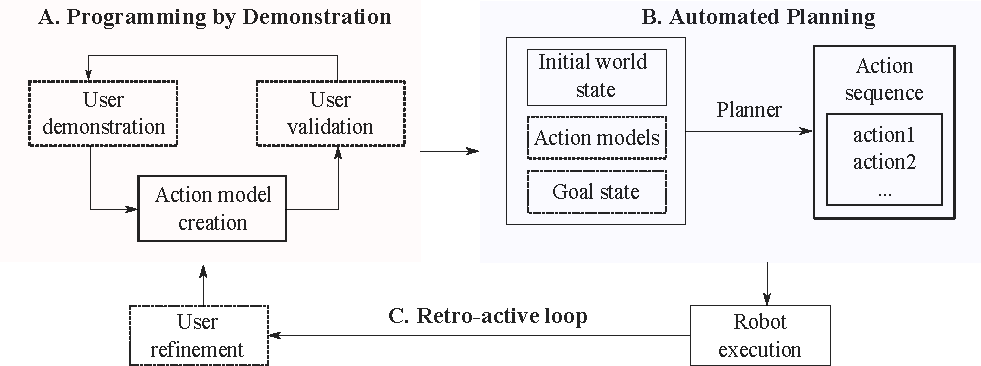
\includegraphics[width=\linewidth]{figures/framework}
	\caption{A robot programming framework for non-expert users: the user teaches action models, which are used by the robot with an automated planner, to generate an action sequence to achieve a goal.
After an unsuccessful robot execution, the user can refine the taught action models (dotted lines indicate user actions, solid lines indicate robot actions).}
	\label{fig:framework}
\end{figure}

\section{Programming by Demonstration: teaching atomic actions}
%Our approach aims at providing end-users with an intuitive way of 
Teaching robots atomic actions consists of learning both \textit{how} and \textit{when} an action should be applied, \ie the low-level (\sect{ssec:lowlevel}) and high-level representations (\sect{ssec:highlevel}) respectively.
We consider an action that consists of both low- and high-level representations as an \textit{action model}.
Programming by demonstration (PbD) techniques provide end-users with an intuitive way to teach the robot action models. %generally consist of an iterative process.

Low-level actions can be learned using Dynamic Movement Primitives (\cite{pastor2009learning}) or mixture models (\cite{calinon2007incremental}), where entire trajectories are learned and generalised.
In keyframe-based PbD (\cite{akgun2012keyframe,alexandrova2014robot}) actions are represented as a sparse sequence of keyframes that can be connected to perform a skill.
%gripper states (open/close) and end-effector poses relative to perceived objects or to the robot's coordinate frame.
Actions can be learned from multiple demonstrations (\cite{niekum2012learning}) or a single demonstration, where poses are assigned heuristically and corrected by the user if needed (\cite{alexandrova2014robot}).

The user can teach multiple manipulation actions and discriminate between them by associating different high-level conditions that specify \textit{when} the robot should use them (\eg actions using claw or suction grippers).
High-level actions are represented similar to planning operators in task planning (\sect{subsec:Classical planning problem}), where an action is represented as a tuple $o = (\text{name}(o), \text{precond}(o),$ $\text{effect}(o))$.
To learn the preconditions and effects, the robot uses a perception system (\eg SIFT (\cite{ahmadzadeh2015learning}) or a database of object features (\cite{mason2011robot})) that recognises object properties in the state of the world.
When the user demonstrates an action, such as pick-and-place of a cube, %\texttt{(move cube A B)}.
it results in a change in the world state, \eg the cube's position.
The robot observes the world state before and after the action demonstration, and extracts the relevant preconditions and effects to build an action model. %, expressed in a symbolic planning language.% (Fig. \ref{fig:action} bottom).
The user validates the learned action model, and provides additional demonstrations if necessary to refine the low- or high-level representations.
Feature-based algorithms, such as k-means clustering (\cite{mollard2015robot,abdo2013learning}), can be used to learn high-level actions from multiple demonstrations.
Existing PbD approaches try to teach the robot from a small number of demonstrations \cite{orendt2016robot,abdo2013learning}, but require at least five contextually different ones.
%To learn object manipulation tasks, the robot perceives the initial world state before %(\textit{precondition}) and after the action demonstration and infers the high-level conditions (\cite{ahmadzadeh2015learning}).
%(\textit{effects}). 
We propose an interactive learning approach, where the user can directly modify and correct the learned action models via the graphical interface.
Thus, the robot can learn a new action from a single demonstration with the user acting as the expert to correct associated conditions.
%The robot learns from multiple demonstrations to generalise trajectories and high-level conditions.
%In the framework, we assume that the learned action trajectory is independent of the trajectory performed by the teacher.

%Note that we do not address the perception problem in this paper. 
%In our experiments, we implemented a simple python algorithm with integrated functionalities of the Robot Operating System (ROS) (\cite{quigley2009ros}), to detect and move objects, based on their colour.


%Table \ref{tab:action-model} shows the states of the demonstrated action and the generalised action model. 
%The generalised operator is automatically translated into a symbolic representation, allowing the creation of a planning domain, without the need for any programming knowledge.


\section{Automated Planning: reusing actions}\label{sec:AP}
Automated planners (\sect{sec:AP}) are used to generate solutions to solve complex problems.
Various planners have been used for task planning with robots, such as the Metric-FF (\cite{cubek2015high}) or the fast downward planner (\cite{abdo2013learning}). 
Given a description of a planning \textit{domain}, \ie object types, predicates, and high-level actions, we can define a planning \textit{problem} with an initial state and a desired goal state to achieve. 
The planner generates an optimal action sequence, or \textit{plan}, which guarantees the transition from initial state to the goal state. 
%Automated planners try to model the robot's strategies, when operating in diverse environments \cite{ghallab2004automated}.
%ught actions are reused with existing task planners by translating them into PDDL (\citet{mcdermott1998pddl}). 
To facilitate the programming process, the framework provides a partial PDDL domain that includes a set of predefined object types and predicates.
In the PbD step, the robot learns action models in the high-level representation that can be used with a planner. 
The user completes the PDDL domain by creating new action models and correcting preconditions and effects via the user interface.
% and manually adding custom types and predicates via the user interface.

The user then creates a new planning problem by detecting the initial world state and defining the goal states to achieve.
The initial world state is automatically recognised by the robot using the same perception system as in the PbD phase. 
The user can modify the detected world states and enter an arbitrary goal for the robot to achieve using the taught action models.
The automated planner generates a plan, consisting of an ordered action sequence for the robot to execute. 
The user can verify the generated plan and have the robot execute it in real life.
If no plan is generated or if the plan seems incorrect, users can modify the taught actions, initial or goal states and relaunch the planner.


\section{Retro-active Loop: refining action models}
The retro-active loop allows the user to revisit and correct created action models.
%Generating a plan under different initial states allows the user to test the created action models.
It is likely that the generated plan does not produce the desired outcome, especially if the context of the planning problem is different to that of the initial demonstration (\eg different object types or positions).
To minimise the user's programming process, taught actions should be generalised and reused as much as possible.
Instead of creating new action models for each problem, the user should revisit and modify existing ones so that they are used correctly by the planner.
Thus, the application to a new context is an important step to test the generalisability of action models.
If the generated plan is incorrect, there are several possible causes:
\begin{itemize}
	\item \textbf{Object types:} they dictate what objects an action can be applied to. If they do not match those of the current planning problem, actions would not be considered by the planner (\eg pick-and-place was only defined for cube objects but not other types).
	\item \textbf{Preconditions:} this can lead to suboptimal or non-existing solutions as the planner makes incorrect assumptions on the allowed usage of taught actions (\eg trying to use a suction gripper on a pointed object).
	\item \textbf{Effects:} similar to preconditions this can lead to suboptimal or non-existing solutions as the world state is not correctly updated after the action execution (\eg a position is still considered free when it is occupied).
	\item \textbf{Initial world state:} if the initial world state is incorrect the planner could consider certain actions as invalid due to preconditions that are required to apply them.
	\item \textbf{Goal states:} it is important to define only the main states that need to be achieved, rather than consequences or intermediate steps to achieve them. Furthermore, contradicting goal states can lead to non-existing plans (\eg an object is on a position and the position is free are states as goal states).
\end{itemize}

Knowledge engineering tools (\sect{subsec:Knowledge Engineering}) facilitate this process of modifying action models used for automated planners.
They often provide useful functionalities for dynamic testing, model checking and visualisation (\cite{simpson2007planning}), where the quality of the models generated does not depend on the user's expertise.
In this thesis we argue that this step does not require expertise in automated planning but can be learned easily by users with different educational backgrounds.